\section{Results}

\subsection{Training comparison}
\begin{figure}[H]
	\centering
	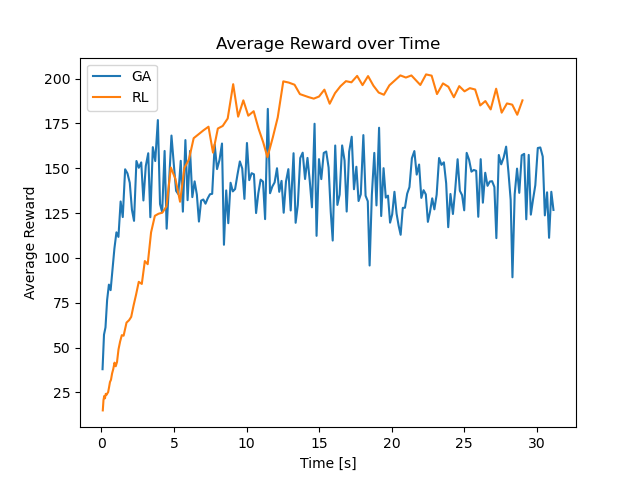
\includegraphics [scale = 0.5]{Images/RL_GA_comparison_avg.png}
	\caption{placeholer}
	\label{figAVG}
\end{figure}

\begin{figure}[H]
	\centering
	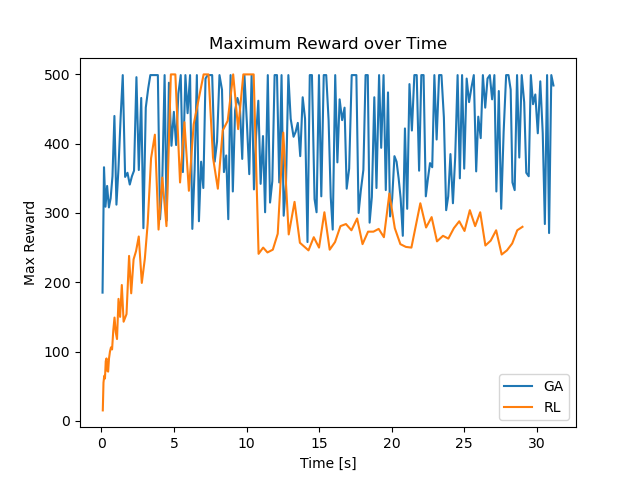
\includegraphics [scale = 0.5]{Images/RL_GA_comparison_max.png}
	\caption{placeholer}
	\label{figMAX}
\end{figure}



\subsection{final model comparison}

The second approach used to compare the obtained results is based on the final models' observations.

Figure \ref{figTABLEDIFF} shows the difference between the two obtained state-action tables of the final reinforcement learning agent and one of the individuals from the last generation of the genetic algorithm.

Since the \textit{Q-Table} does not provide an exact chosen action given a state, the compared state-action table of the reinforcement learning agent used in Figure \ref{figTABLEDIFF} is obtained by selecting the action $a$ of the state $s$ as $a = argmax_{a_i} (Q(s,a_i))$.

\begin{figure}[H]
	\centering
	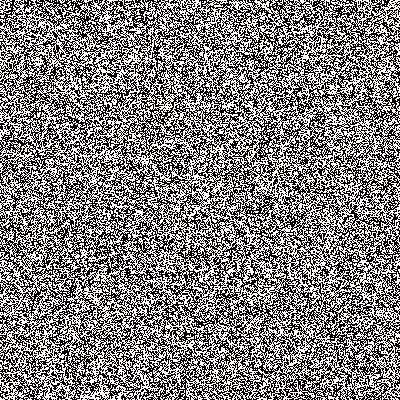
\includegraphics [scale = 0.7]{Images/diff.png}
	\caption{Difference between the two state-action tables obtained using GA and RL. The black pixels represent the states where the chosen action is the same, while white pixels represent a different action choice. The x-axis contains all the possible pairs of the first two elements of the state's 4D-vector, $(s_1,s_2)$, and the y-axis contains all the possible pairs of the last two elements, $(s_3,s_4)$. }
	\label{figTABLEDIFF}
\end{figure}

Looking into Figure \ref{figTABLEDIFF}, it is possible to observe how the actions selected by the two algorithms differ in various states. However, some wide areas where the action taken by both algorithms is the same can be spotted, which could be referred to as sensitive states where considering a different choice could lead the pole to fall down.\\

Figure \ref{figRLvsGA} shows the final testing results of the two methods. As already showed by the traning comparison in both figure \ref{figAVG} and figure \ref{figMAX}, The reinforcement learning agent showed a better generalization ability and more understanding of the environment, leading to obtain better results.\\
The testing has been conducted as follow: the environment has been seeded with ten different seeds and for every execution the same environment has been provided to both the algorithm.
The reinforcement learning agent has been tested using the obtained \textit{q-table} from the training, the genetic algorithm population is the last generation of the training performed.\\
Every individual of the GA population have been tested for all the tests, and the best one has been considered for the comparison, during the testing of the population, no particular difference have been noticed between the reward obtained by the individuals.

\begin{figure}[H]
	\centering
	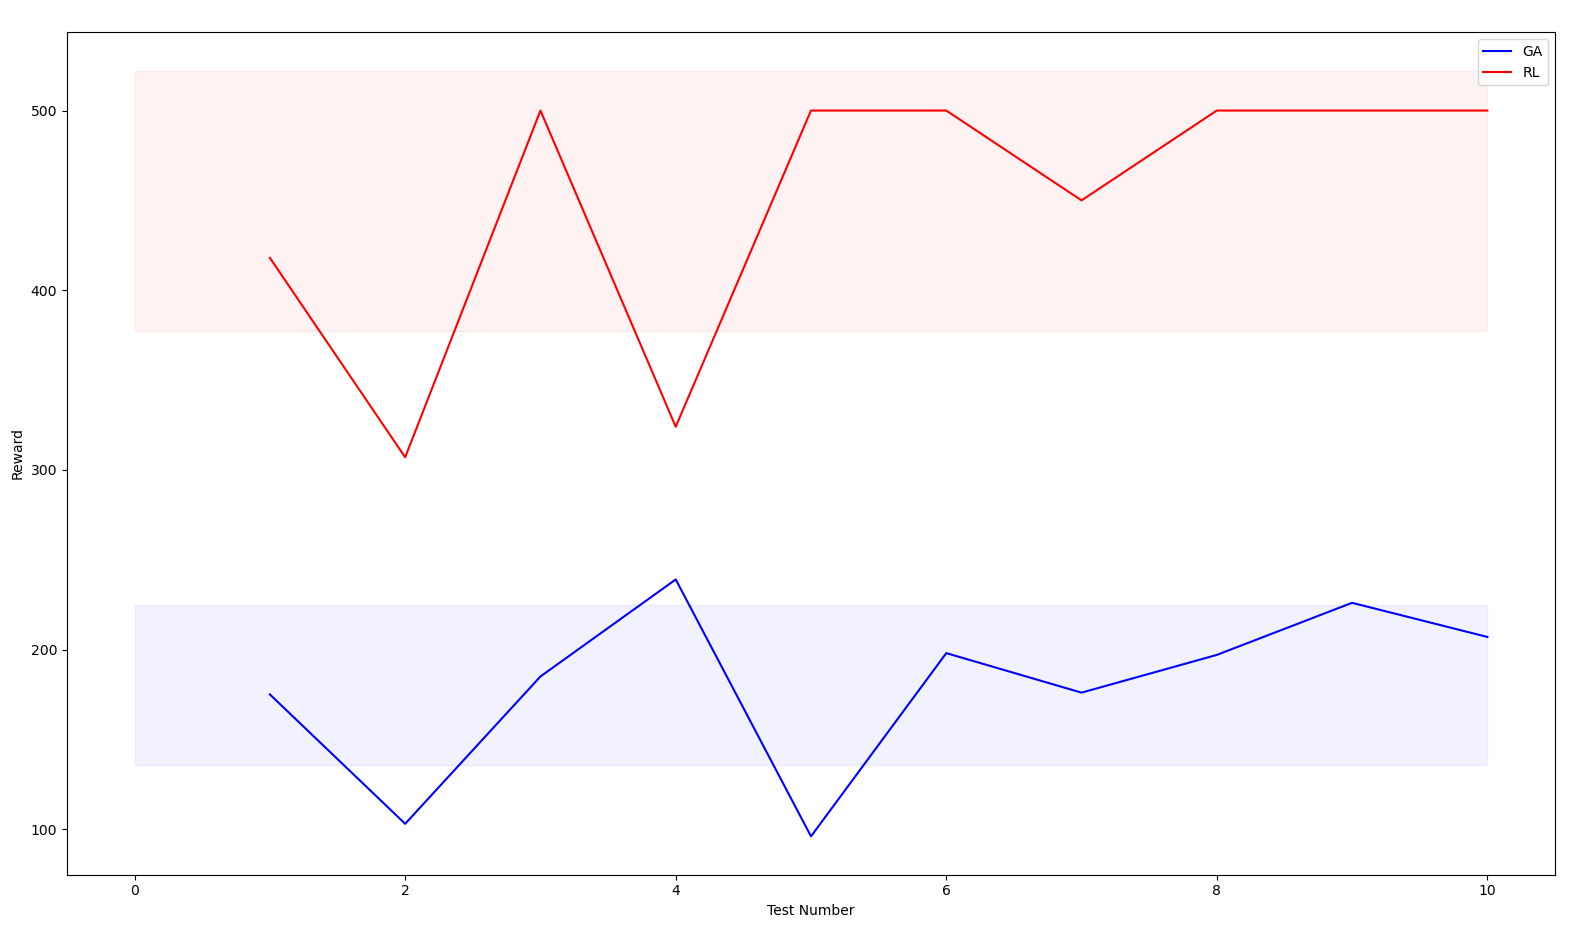
\includegraphics [width=0.5\textwidth]{Images/GAvRL_backup.png}
	\caption{The plot shows the results obtained testing the two models on the same test set. The x-axis represents the number of the test set, the y-axis the number of steps the model was able to take before reaching the goal. The blue line represents the results obtained using the model trained with the GA, the red line the results obtained using the model trained with the RL.}
	\label{figRLvsGA}
\end{figure}

Observing the results, some differences regarding the variance can be noticed: the GA population seem to obtain more consistent results in different tests, but due the fact that the testing is performed on the entire generation this could be related to the fact that every time the best individual is extracted.\\
	
\textcolor{blue}{To describe the differences between the two gifs below here :)}
	
% RL FRAMES %
\begin{figure}[H]
	\centering
	\begin{subfigure}
		\centering
		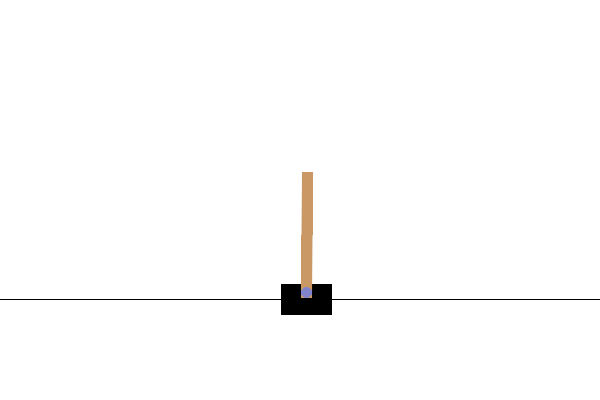
\includegraphics[width=0.3\linewidth]{Images/frames/RL/1.png}
	\end{subfigure}
	\hfill
	\begin{subfigure}
		\centering
		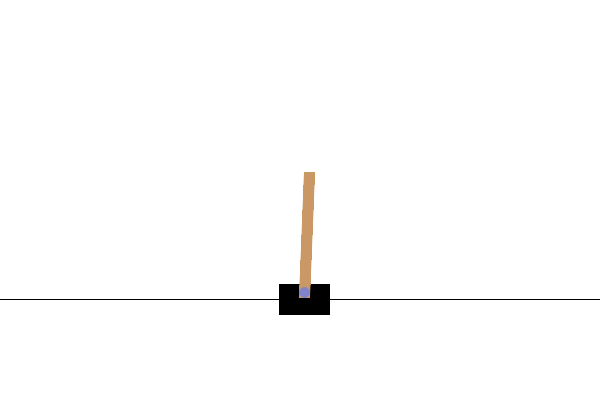
\includegraphics[width=0.3\linewidth]{Images/frames/RL/2.png}
	\end{subfigure}
	\hfill
	\begin{subfigure}
		\centering
		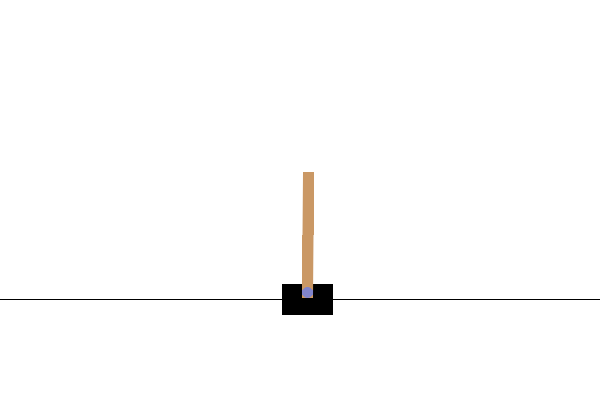
\includegraphics[width=0.3\linewidth]{Images/frames/RL/3.png}
	\end{subfigure}
	\\
	\begin{subfigure}
		\centering
		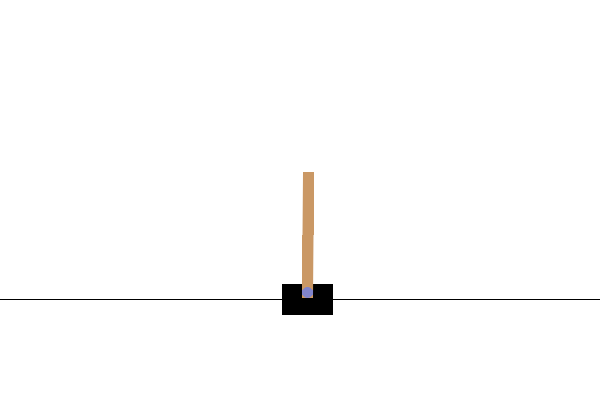
\includegraphics[width=0.3\linewidth]{Images/frames/RL/4.png}
	\end{subfigure}
	\hfill
	\begin{subfigure}
		\centering
		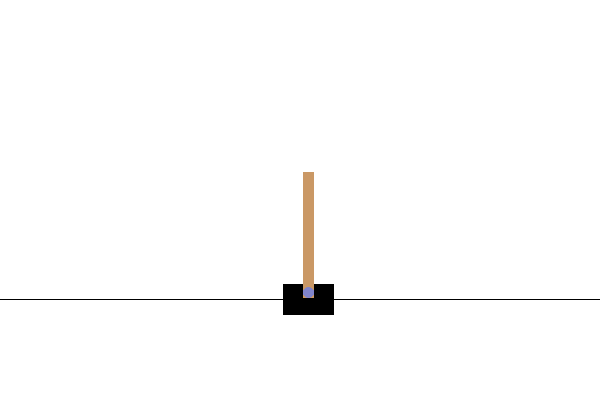
\includegraphics[width=0.3\linewidth]{Images/frames/RL/5.png}
	\end{subfigure}
	\hfill
	\begin{subfigure}
		\centering
		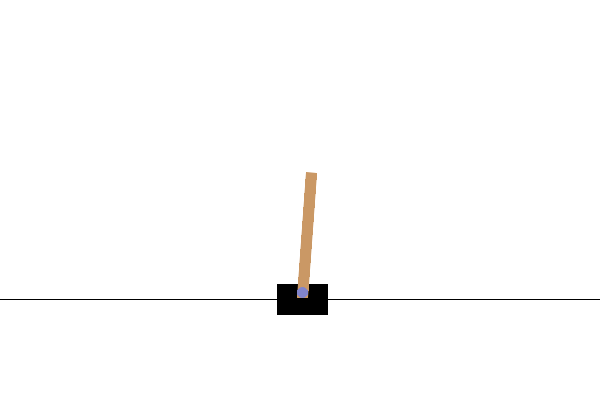
\includegraphics[width=0.3\linewidth]{Images/frames/RL/6.png}
	\end{subfigure}
	\\
	\begin{subfigure}
		\centering
		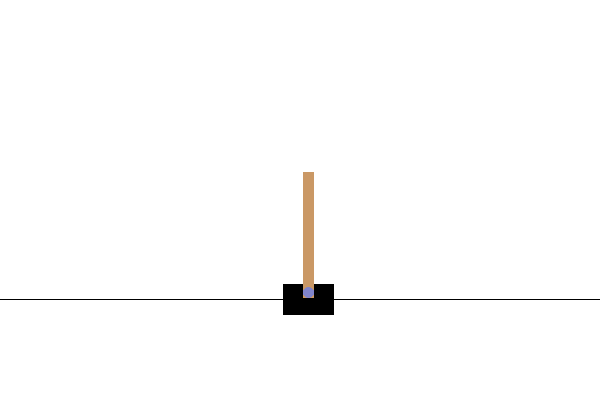
\includegraphics[width=0.3\linewidth]{Images/frames/RL/7.png}
	\end{subfigure}
	\hfill
	\begin{subfigure}
		\centering
		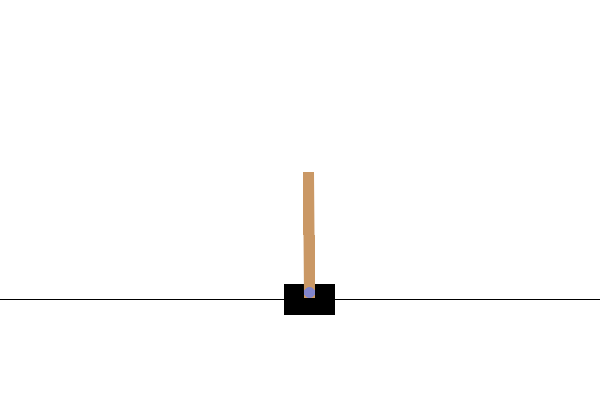
\includegraphics[width=0.3\linewidth]{Images/frames/RL/8.png}
	\end{subfigure}
	\hfill
	\begin{subfigure}
		\centering
		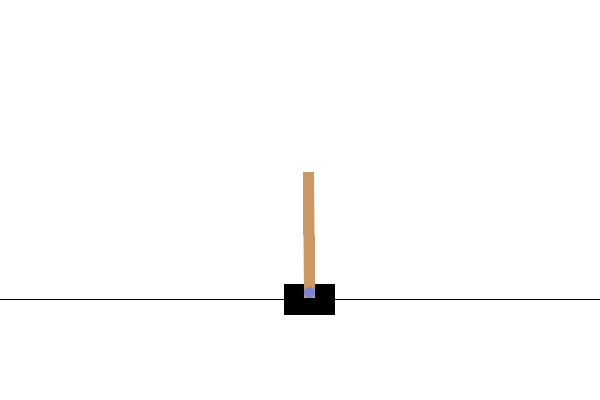
\includegraphics[width=0.3\linewidth]{Images/frames/RL/9.png}
	\end{subfigure}
	\\
	\begin{subfigure}
		\centering
		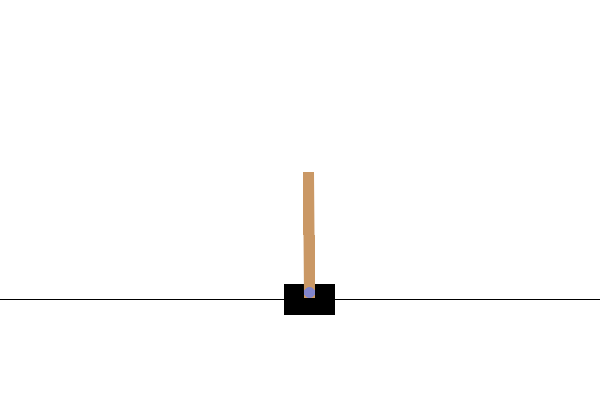
\includegraphics[width=0.3\linewidth]{Images/frames/RL/10.png}
	\end{subfigure}
	\hfill
	\begin{subfigure}
		\centering
		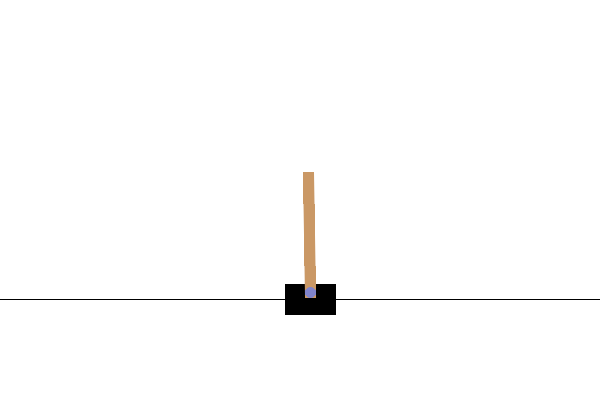
\includegraphics[width=0.3\linewidth]{Images/frames/RL/11.png}
	\end{subfigure}
	\hfill
	\begin{subfigure}
		\centering
		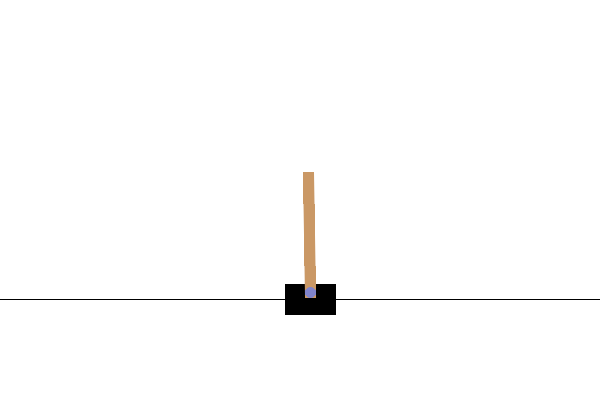
\includegraphics[width=0.3\linewidth]{Images/frames/RL/12.png}
	\end{subfigure}
	\caption{Frames RL}
	\label{fig:framesRL}
\end{figure}
% GA FRAMES %

\begin{figure}[H]
	\centering
	\begin{subfigure}
		\centering
		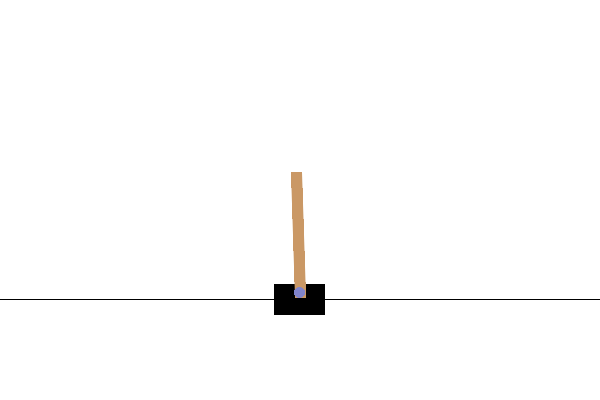
\includegraphics[width=0.3\linewidth]{Images/frames/GA/1.png}
	\end{subfigure}
	\hfill
	\begin{subfigure}
		\centering
		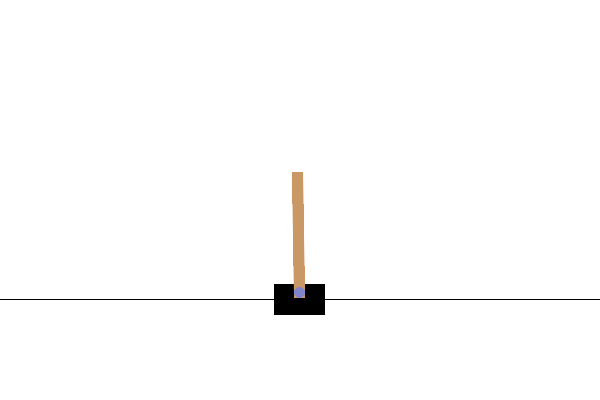
\includegraphics[width=0.3\linewidth]{Images/frames/GA/2.png}
	\end{subfigure}
	\hfill
	\begin{subfigure}
		\centering
		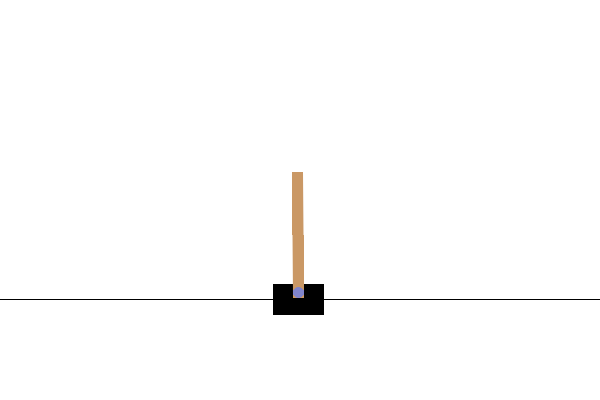
\includegraphics[width=0.3\linewidth]{Images/frames/GA/3.png}
	\end{subfigure}
	\\
	\begin{subfigure}
		\centering
		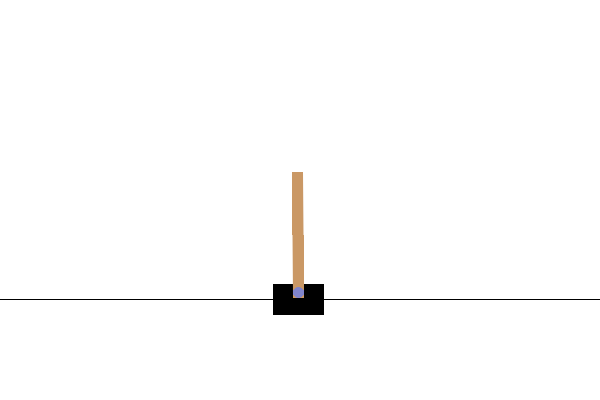
\includegraphics[width=0.3\linewidth]{Images/frames/GA/4.png}
	\end{subfigure}
	\hfill
	\begin{subfigure}
		\centering
		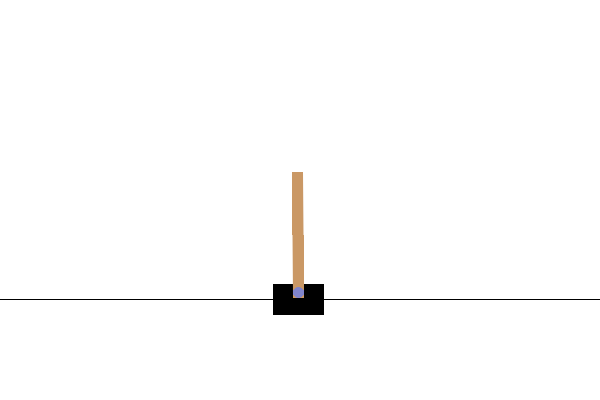
\includegraphics[width=0.3\linewidth]{Images/frames/GA/5.png}
	\end{subfigure}
	\hfill
	\begin{subfigure}
		\centering
		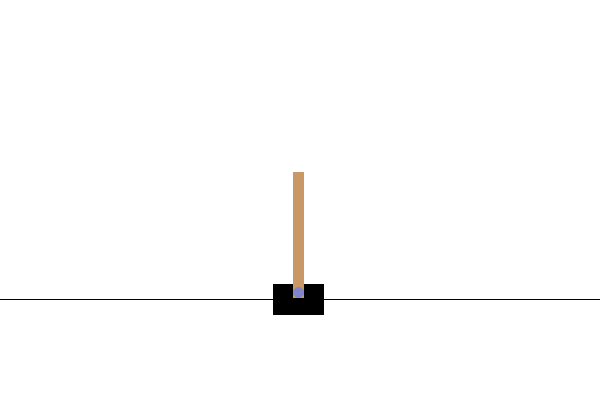
\includegraphics[width=0.3\linewidth]{Images/frames/GA/6.png}
	\end{subfigure}
		\\
	\begin{subfigure}
		\centering
		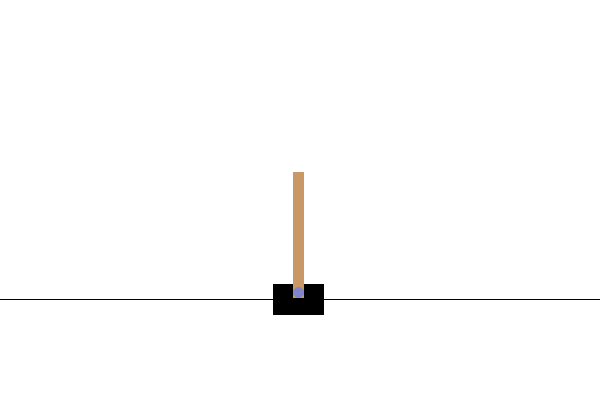
\includegraphics[width=0.3\linewidth]{Images/frames/GA/7.png}
	\end{subfigure}
	\hfill
	\begin{subfigure}
		\centering
		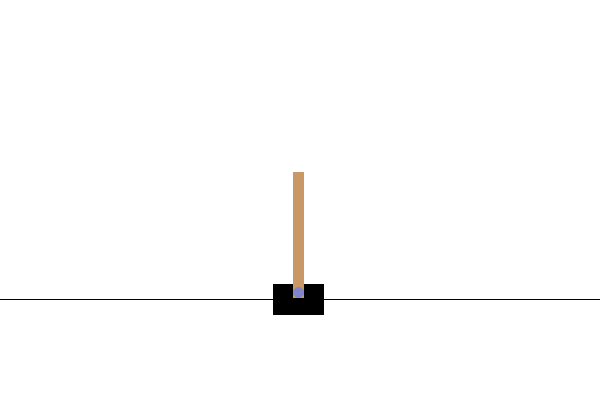
\includegraphics[width=0.3\linewidth]{Images/frames/GA/8.png}
	\end{subfigure}
	\hfill
	\begin{subfigure}
		\centering
		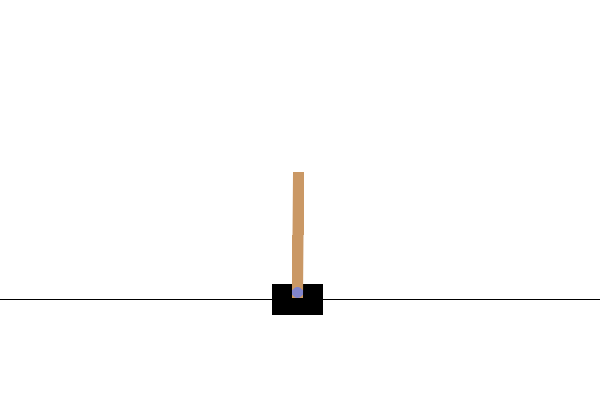
\includegraphics[width=0.3\linewidth]{Images/frames/GA/9.png}
	\end{subfigure}
	\\
	\begin{subfigure}
		\centering
		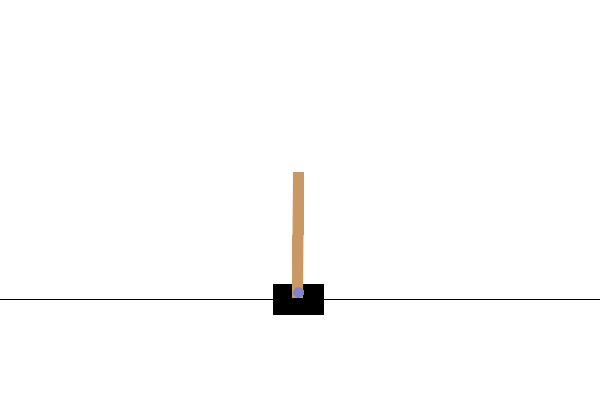
\includegraphics[width=0.3\linewidth]{Images/frames/GA/10.png}
	\end{subfigure}
	\hfill
	\begin{subfigure}
		\centering
		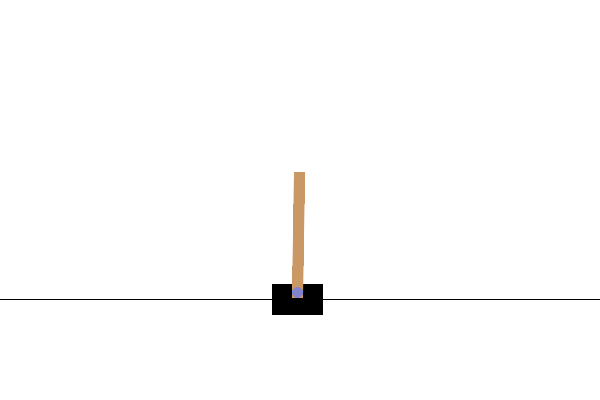
\includegraphics[width=0.3\linewidth]{Images/frames/GA/11.png}
	\end{subfigure}
	\hfill
	\begin{subfigure}
		\centering
		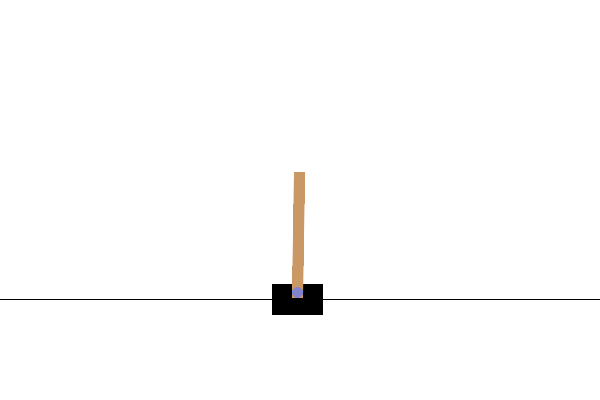
\includegraphics[width=0.3\linewidth]{Images/frames/GA/12.png}
	\end{subfigure}
	\caption{Frames GA}
	\label{fig:framesGA}
\end{figure}


	



% % Delete the text and write your Results here:
% %------------------------------------

% The results section can be combined with the discussion if appropriate. In case of many sub\-/experiments % \-/ fixes the problem that LaTeX won't hyphenate words with dashes in them.
% where the results are vaguely related or unrelated, it would be appropriate to combine the results and discussion. This way you have the information related to each sub-experiment gathered in one place. \par
% Provide uncertainties for the results, but don't discuss it. Do not involve personal opinions, just present the cold hard results in form of numbers, tables, graphs and some sentences. \par
% \Cref{tab:Some-numbers} shows a nice table with comma alignment. \par

% \begin{table}[htb]%
% \centering
% \caption{Table with comma alignment.}
% 	\label{tab:Some-numbers}
% 	\begin{tabular}{SSS} 		% S = special column format from the siunitx package. Aligns commas.
% 		\toprule
% 		{$m$}  &  {$a$}  & {$F$}  \\
% 		{(\si{kg})} &  {(\si{m.s^{-2}})} & {(\si{N})}  \\
% 		\midrule
% 		1,2 & 10,1 & 12 \\
% 		2,44 & 6,92 & 16,88 \\
% 		10 & 1,0 & 10 \\
% 		8,2 & 1,1 & 9,0 \\
% 		100 & 1 & 100 \\
% 		\bottomrule
% 	\end{tabular}
% \end{table}

